\documentclass[a4paper,12pt]{mwart}

\usepackage[polish,english]{babel}
\usepackage[utf8]{inputenc}
\usepackage{polski}
\usepackage[T1]{fontenc}
\usepackage{indentfirst}
\frenchspacing

\usepackage{enumerate}
\usepackage{csquotes}
\usepackage{graphicx}
\usepackage{float}
\usepackage{makecell}
\usepackage{siunitx}
\sisetup{output-decimal-marker = {,}}
\usepackage{icomma}
\let\lll\undefined
\usepackage{amsmath, amssymb, amsfonts}
\usepackage{mathtools}
\usepackage{setspace}
\usepackage{import}

\usepackage[%
style=numeric,
sorting=none,
backend=biber,
language=autobib,
autolang=other,
]{biblatex}

\addbibresource{bibliografia.bib}

\begin{document}

\onehalfspacing
\begin{flushleft}

  \textbf{Szymon \MakeUppercase{Mikulicz}} \\
  \textbf{Marcel \MakeUppercase{Piszak}} \\
  \vspace*{12pt}

  \MakeUppercase{\textbf{Wibroakustyczna stacja pomiarowa oparta o mikrokomputer Raspberry Pi}} \\
  \vspace*{6pt}
  \MakeUppercase{\textbf{Vibroacoustic measuring station based on Raspberry Pi microcomputer}} \\
  \vspace*{12pt}

  AGH Akademia Górniczo-Hutnicza \\
  Wydział Inżynierii Mechanicznej i Robotyki \\
  Katedra Mechaniki i Wibroakustyki \\
  \vspace*{6pt}

  czilukim@o2.pl \\
  marcel.piszak@wp.pl \\

\end{flushleft}

\noindent
\textbf{Streszczenie} \\
Treść streszczenia
\vspace*{24pt}

\noindent
\textbf{Abstrakt} \\
Współczesne rozwiązania dedykowane do pomiarów drgań budynków proponowane przez
popularnych producentów sprzętu pomiarowego charakteryzują się dużym stopniem
skomplikowania. Celem niniejszego projektu było zbudowanie prostego i
przystępnego cenowo systemu pozwalającego na pomiar i analizę drgań budynków
zgodną z normą PN-B 02170:2016-12. Postanowiono stworzyć system pomiarowy
oparty na platformie Raspberry Pi® oraz wykorzystujący akcelerometry typu MEMS
w celu minimalizacji kosztów i rozmiarów stacji. Oprogramowanie kontrolujące
akwizycję oraz analizę danych napisano przy użyciu języka Python i odpowiednich
bibliotek. Skonstruowanie oraz uruchomienie zaprogramowanego układu ma
bezpośrednio przyczynić się do realizacji większego projektu obejmującego
połączenie takich jednostek analizujący drgania na większym obszarze.
\vspace*{24pt}


\section{Wstęp}

Pomiary drgań są ważnym elementem oceny wibroakustycznej w technice. Jednym
z wielu pól na których można je stosować jest badanie wpływu wibracji
podłoża na budynki. Źródła drgań oddziałujące na obiekty budowlane są
zróżnicowane, ale najczęściej pochodzą od wszelkich środków transportu
eksploatowanych w bezpośredniej bliskości zabudowy. W miastach wzmożona
komunikacja samochodowa, ruch tramwajowy, a nawet metro potrafią powodować
występowanie drgań o dużych amplitudach przyspieszeń. Z kolei konstrukcje
budynków poddawane długotrwałej ekspozycji na drgania mogą ulegać
uszkodzeniom, a w skrajnych przypadkach zniszczeniu. Dodatkowo na terenach
miejskich często można spotkać budynki wymagające dużego ograniczenia wpływu
drgań za względu na pełnione funkcje. Różnego rodzaju laboratoria, szpitale
czy przemysł precyzyjny nie dopuszczają występowania drgań o amplitudach
uniemożliwiających pełnienie danej funkcji przez mieszczący je budynek.

Istnieją różne metody pomiaru oraz analizy drgań oddziałujących na budynki
jednak pewne dokumenty normatywne pozwalają na określenie wpływu drgań oraz
weryfikację pomiarową i późniejsze porównania, czy też odniesienie wyników
do wartości dopuszczalnych. Norma PN-B 02170:2016-12 pod tytułem ,,Ocena
szkodliwości drgań przekazywanych przez podłoże na budynki'' \cite{norma}
zawiera przede wszystkim metodykę oceny wpływu drgań, ale można w niej
znaleźć również unormowane zasady wykonywania pomiarów.

\section{Przegląd dostępnych rozwiązań}

Na przestrzeni ostatnich lat popularne stało się wykorzystanie platform
komputerowych wspierających naukę programowania takich jak Arduino czy Raspberry
Pi do tworzenia wszelkiego rodzaju jednostek pomiarowych. Takie aplikacje
znajdują również zastosowania w pomiarach wibroakustycznych. Platforma Raspberry
Pi, ponieważ w zasadzie jest samodzielnym komputerem z systemem operacyjnym
opartym na jądrze Linux, daje duże możliwości tworzenia samodzielnych systemów
pomiarowych. Do tej pory dominującym podejściem pomiarowym drgań oraz hałasu
jest wykorzystanie analogowego przetwornika będącego osobnym elementem toru
pomiarowego. Sygnał analogowy jest przesyłany z reguły do karty pomiarowej, a
następnie, pod postacią cyfrową, trafia do komputera który jest odpowiedzialny
za jego analizę. W wielu przypadkach duża dokładność pomiaru wymusza
zastosowanie profesjonalnych, wyspecjalizowanych przetworników, ale niekiedy
zdarza się, że sygnał pomiarowy nie wymaga bardzo dużej rozdzielczości lub
częstotliwości próbkowania. Podejmowano już pracę nad stworzeniem systemów
analizy drgań opartym na platformie Raspberry Pi \cite{art1}. Autorzy publikacji
skupili się na opracowaniu systemu monitorowania i analizy drgań na podstawie
widma, tak aby łatwo dało się go dostosować do środowiska działania. 

\section{Założenia projektowe}

Głównym założeniem projektu była prostota konstrukcji, dostępność elementów i
ich zgodność z wymogami pomiarów określonych w normie \cite{norma}. Charakter
sygnału drgań mierzonego na potrzeby normy określają następujące parametry:
\begin{itemize}
  \item Pasmo częstotliwości od \SI{0,5}{\hertz} do \SI{100}{\hertz}
  \item Amplituda prędkości drgań od \SI{e-4}{\metre\per\second} do \SI{1}{\metre\per\second}
  \item Amplituda przyspieszenia drgań od \SI{e-3}{\metre\per\square\second} do \SI{10}{\metre\per\square\second}
\end{itemize}
Norma wskazuje również na posiadanie możliwości zapisu w pamięci urządzenia
zarejestrowanych wibrogramów. Analiza powinna być prowadzona w pasmach
tercjowych. W procesie przetwarzania i analizy sygnału wykorzystano wyłącznie
biblioteki na licencji wolnego oprogramowania, a cały kod napisany podczas jego
realizacji umieszczono na platformie GitHub.

\section{Opis realizacji projektu}

Stacja pomiarowa będąca przedmiotem niniejszego projektu została oparta o
platformę Raspberry Pi 3 model B. Jako czujnik drgań wybrano moduł akcelerometru
MEMS MMA8451 firmy Adafruit. Jest on niewielkich rozmiarów, pozwala na pomiar
przyspieszenia drgań w trzech osiach. Posiada wbudowany, 14-bitowy przetwornik
analogowo-cyfrowy oraz ma możliwość komunikacji z mikroprocesorem za pomocą
interfejsu I\textsuperscript{2}C. Warto także zaznaczyć, że akcelerometr ten
pozwala na wybór jednego z trzech dostępnych zakresów pomiarowych:
$\pm$\SI{2}{\g}, $\pm$\SI{4}{\g} oraz $\pm$\SI{8}{\g}. Częstotliwość próbkowania
także może być zmieniana przez użytkownika, a jej największa wartość to
\SI{800}{\hertz}. Akcelerometr posiada również wiele wbudowanych funkcji, między
innymi filtr górnoprzepustowy.

Jako system operacyjny dla mikrokomputera wybrano Rasbian -- przygotowaną
specjalnie dla Raspberry Pi dystrybucję Linuxa. Wybrano wersję Lite, jedynie z
obsługą z poziomu terminala. Komunikacja z komputerem pozwalająca na
oprogramowanie oraz obsługę stacji odbywała się przez protokół SSH.
Mikrokomputer posada zarówno złącze Ethernet jak i moduł Wi-Fi, co umożliwia
podłączenie go do sieci LAN.

\begin{figure}[H]
  \centering
  \import{vecgraphics/}{schemat.pdf_tex}
  \caption{Schemat stworzonego systemu pomiarowego}
  \label{fig:schemat}
\end{figure}

\begin{figure}[H]
  \centering
  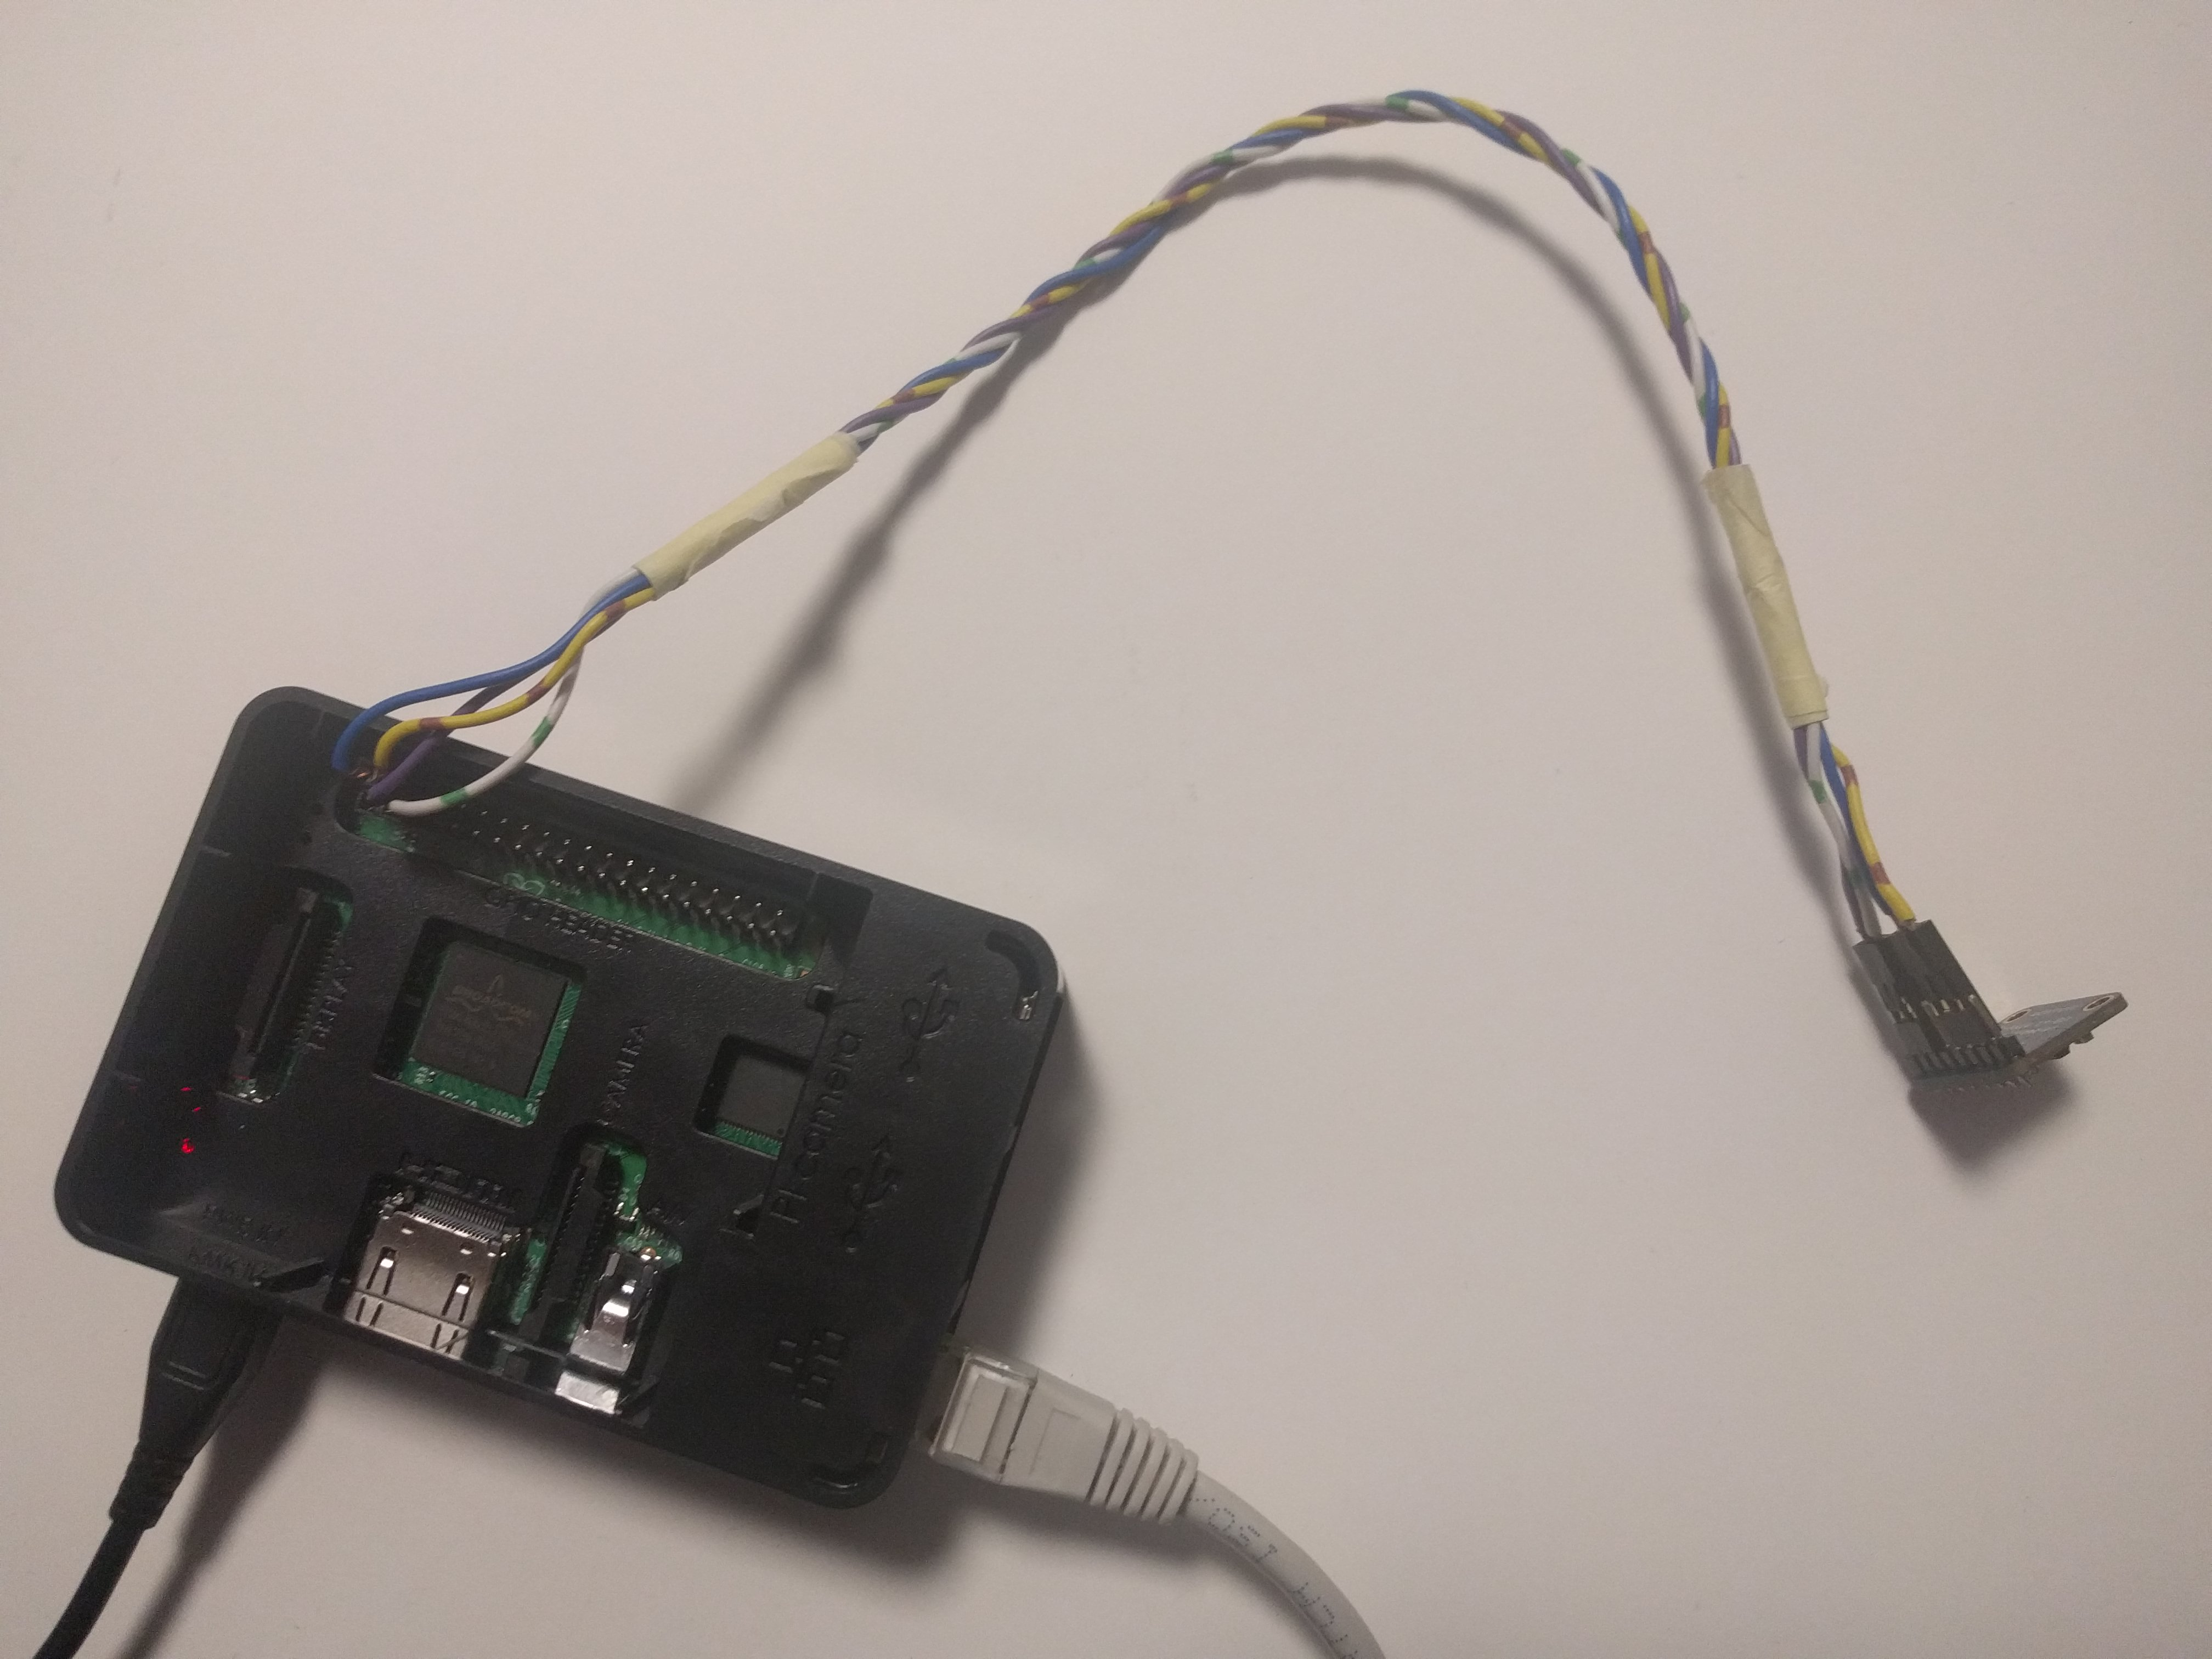
\includegraphics[width=\textwidth]{bitgraphics/pi.png}
  \caption{Wibroakustyczna stacja pomiarowa}
  \label{fig:foto}
\end{figure}
% opis kodu

Stacja pomiarowa jest zdolna do zapisania w swojej pamięci wewnętrznej około X
godzin wibrogramu. Ponieważ norma wymaga analizy tercjowej drgań, uwzględniono
filtrację sygnału w pasmach od \SI{0,5}{\hertz} do \SI{100}{\hertz}.

% przykładowe pomiary

\section{Wnioski}

% wnioski ogólne i dotyczące wyników

Należy pamiętać, że projekt ten jest częścią większego, mającego objąć swoim
zakresem pomiary zarówno drgań jak i hałasu środowiskowego. Stacje pomiarowe
wyposażone w akcelerometry oraz mikrofony rejestrowałyby dane, a następnie
wysyłały je na serwer sieciowy, gdzie byłyby one analizowane oraz przechowywane.
Dostęp do nich byłby możliwy przez aplikację hosta, gdzie można by było
przeglądać dane aktualne oraz analizować dane archiwalne.

\printbibliography

\end{document}
